\chapter{Results}
\section{Cumulative apparent fishing hours}
A total of 213 unique longliners and purse seiners were recorded for 2015-2024. These vessels
together accounted for an average of 122 760 hours per year, with an average of 576 hours per
vessel per year. Areas that show the highest effort throughout the study time include the
Mediterranean coast of Spain, around Sardinia and Sicily, south of Malta, the Adriatic, and south
of Cyprus \figref{sub0:fig:sum_cv}. Areas with high effort generally also show the lowest
coefficient of variation \figref{sub1:fig:sum_cv}. There does not appear to be any fishing activity
based on AIS around the African Mediterranean coast \figref{fig:sum_cv}.

\medskip

\begin{figure}[ht]
	\subplot{2}
	{width=1\linewidth, trim=1.2cm 0 1.2cm 0,clip}
	{Figures/plots/sum_cv.pdf}
	{%
		Summary statistics for both longliners and purse-seiners. \subref{sub0:fig:sum_cv}) Cumulative fishing hours in the Mediterranean (2015-2024).
		Colors are on a log-scale. \subref{sub1:fig:sum_cv}) Coefficient of variation between years (standard deviation divided by mean) for each cell.
	}{fig:sum_cv}
\end{figure}

\FloatBarrier
\section{Fishing hotspots and high risk areas}
Numerous persistent longline hotspot areas were identified throughout the Mediterranean including
the southern coast of Spain, south of Sardinia, around Sicily and Malta, as well as south of Cyprus
\figref{sub0:fig:longline_hotspots}. These hotspots show however, differing trends. Fishing hours
in the south of Malta appear to be increasing throughout, with a similar trend of increase in the
Adriatic Sea. Other areas that appear to be consistent hotspots, like the east of Sicily, show a
decreasing trend \figref{sub1:fig:longline_hotspots}.

\begin{figure}[H]
	\subplot{2}
	{width=1\linewidth, trim=0.85cm 0 1.2cm 0,clip}
	{Figures/plots/dll_hotspot_trend.pdf}
	{%
		Hotspot percentage and trend scores for longliners in the Mediterranean.
		The percentage reflects the years in which a given cell was a hotspot based on the Getis-Ord Gi* statistic.
		The Z-score is derived from the Mann-Kendall statistic.}
	{fig:longline_hotspots}
\end{figure}

Purse seine hotspots appear persistent around the Balearic Islands, in the Adriatic Sea, and along
the Calabrian coast in Italy \figref{sub0:fig:seines_hotspots}. Trends in these areas show a clear
increase around Ibiza and in the central Adriatic, while areas around the coast in the Adriatic
show a decrease \figref{sub1:fig:seines_hotspots}. The hotspot area along Calabria shows no clear
trend.

\begin{figure}[ht]
	\subplot{2}
	{width=1\linewidth, trim=0.4cm 0 0.7cm 0,clip}
	{Figures/plots/pss_hotspot_trend.pdf}
	{%
		Hotspot percentage and trend scores for purse seiners in the Mediterranean.
		The percentage reflects the years in which a given cell was a hotspot based on the Getis-Ord Gi* statistic.
		The Z-score is derived from the Mann-Kendall statistic.}
	{fig:seines_hotspots}
\end{figure}

\FloatBarrier
\section{Temporal changes}
Longline fishing hours show a clear seasonal trend where activity is highest during warmer months
(mainly in the summer) and lowest in the colder months around winter
\figref{sub0:fig:longlines_ridge}. Some areas show high effort earlier in the season in spring (for
example south of Malta) and others are more persistent later in the season in fall (for instance
around Ibiza). The time series show a similar seasonal trend, although the intensity varies between
years, and it appears that the longline season is expanding between years
\figref{sub1:fig:longlines_ridge}. The highest annual longline fishing hours throughout the study
time were recorded for 2022 and the lowest for 2015 \tabref{tab:year_hours}.

\begin{figure}[htp]
	\customsubplot{2}
	{1\linewidth}                           % width
	{0.5cm 0 0.6cm 0}                       % trim
	{Figures/plots/longlines_ridge_seasons.pdf} % file
	{5,92}                                  % (A) position
	{5,40}                                  % (B) position
	{fig:longlines_ridge}
	{%
		Temporal changes in longline fishing hours. \subref{sub0:fig:longlines_ridge}) Spatial differences between seasons.
		Hours are summed per season and cell and colour is on a log-scale. Seasons are defined based on calendar dates:
		winter (Dec 21 - Mar 19), spring (Mar 20 - Jun 20), summer (Jun 21 - Sep 21), and fall (Sep 22 - Dec 20). \subref{sub1:fig:longlines_ridge})
		Time series of fishing hours, summed per year and day.}
\end{figure}

\begin{table}[ht]
	\centering
	\caption{Annual sum of fishing hours for purse seiners and longliners.}
	\medskip
	\begin{tabular}{lcc}
		\toprule
		\textbf{Year} & \multicolumn{2}{c}{\textbf{Fishing hours}}                       \\
		\cmidrule(lr){2-3}
		              & \textbf{Purse seiners}                     & \textbf{Longliners} \\
		\midrule
		2015          & 4,193                                      & 71,846              \\
		2016          & 5,313                                      & 89,136              \\
		2017          & 5,901                                      & 107,345             \\
		2018          & 6,128                                      & 106,130             \\
		2019          & 5,931                                      & 113,261             \\
		2020          & 5,636                                      & 124,927             \\
		2021          & 5,706                                      & 133,361             \\
		2022          & 5,675                                      & 149,059             \\
		2023          & 5,085                                      & 139,068             \\
		2024          & 6,661                                      & 137,406             \\
		\bottomrule
	\end{tabular}
	\label{tab:year_hours}
\end{table}

Regarding the purse seine fleet, fishing hours show a very pronounced seasonal trend with a peak in
spring \figref{fig:seines_ridge}. The core areas of the fishery during spring are the Balearic
Islands, along the coast of Calabria (south-west Italy), and the central Adriatic. In the Adriatic,
there appears to be purse seine activity throughout the whole year \figref{sub0:fig:seines_ridge}.
The purse seine season for large-pelagic species is limited to the months of May and June and is
consistent between years \figref{sub1:fig:seines_ridge}. Highest annual fishing hours for purse
seiners were recorded in 2024 and the lowest in 2015 \tabref{tab:year_hours}.

\begin{figure}[ht]
	\customsubplot{2}
	{1\linewidth}
	{1.2cm 0 0.9cm 0}                       % trim
	{Figures/plots/purse_seines_ridge_seasons.pdf} % file
	{3,93.5}                                  % (A) position
	{3,42}                                  % (B) position
	{fig:seines_ridge}
	{%
		Temporal changes in purse seine fishing hours. \subref{sub0:fig:seines_ridge}) Spatial differences between seasons. Seasons are defined based on calendar dates:
		winter (Dec 21 - Mar 19), spring (Mar 20 - Jun 20), summer (Jun 21 - Sep 21), and fall (Sep 22 - Dec 20).
		Hours are summed per season and cell and colour is on a log-scale. \subref{sub1:fig:seines_ridge}) Time series of fishing hours, summed per year
		and day.}
\end{figure}

\FloatBarrier
\section{Flag countries}

Vessels were flagged to a total of 10 countries and the majority of vessels analysed were
longliners (Tab.~\ref{tab:countries_vessels}; see Fig.~\ref{fig:longline_effort_countries}
and~\ref{fig:seine_effort_countries} for an overview by country). Italy shows the highest amount of
both purse seiners and longliners identified in the GFW data.

\medskip

\begin{table}[ht]
	\centering
	\caption{Number of vessels by country and gear type in 2024 from our detections compared to vessels with drifting longlines currently registered with the GFCM and
		tuna purse seine vessels currently registered with ICCAT. ‘--’ indicates no recorded vessels for that gear. PS = purse seiners, LL = longliners}
	\medskip
	\begin{tabularx}{\textwidth}{l *{6}{>{\centering\arraybackslash}X}}
		\toprule
		\textbf{Country}      & \textbf{Detected PS} & \textbf{Reg. PS} & \textbf{\% PS}  & \textbf{Detected LL} & \textbf{Reg. LL} & \textbf{\% LL}  \\
		\midrule
		Albania               & --                   & 2                & 0.0\%           & --                   & --               & --              \\
		Algeria               & 3                    & 39               & 7.7\%           & --                   & --               & --              \\
		EU-Croatia            & 2                    & 3                & 66.7\%          & --                   & --               & --              \\
		EU-Cyprus             & --                   & 1                & 0.0\%           & 14                   & 15               & 93.3\%          \\
		Egypt                 & --                   & 2                & 0.0\%           & --                   & --               & --              \\
		EU-France             & 13                   & 21               & 61.9\%          & --                   & 4                & 0.0\%           \\
		EU-Greece             & --                   & --               & --              & 8                    & 24               & 33.3\%          \\
		EU-Italy              & 16                   & 19               & 84.2\%          & 60                   & 83               & 72.3\%          \\
		EU-Malta              & --                   & 2                & 0.0\%           & 19                   & 17               & 111.8\%         \\
		Libya                 & --                   & 15               & 0.0\%           & --                   & --               & --              \\
		Morocco               & 1                    & 5                & 20.0\%          & --                   & --               & --              \\
		EU-Spain              & 5                    & 7                & 71.4\%          & 22                   & 30               & 73.3\%          \\
		Tunisia               & --                   & 59               & 0.0\%           & --                   & --               & --              \\
		Turkey                & --                   & 36               & 0.0\%           & --                   & --               & --              \\
		\midrule
		\textbf{Total / Mean} & \textbf{40}          & \textbf{213}     & \textbf{30.1\%} & \textbf{123}         & \textbf{173}     & \textbf{58.6\%} \\
		\bottomrule
	\end{tabularx}
	\label{tab:countries_vessels}
\end{table}

Most regions with high fishing activity are fishing grounds shared by multiple countries
\figref{fig:no_countries}. Regions with high overlap between flag countries for longliners include
the Balearic Islands, south of Crete, and south of Malta, which are also areas with high fishing
hours \figref{sub0:fig:sum_cv}. For purse seiners, fishing generally is more concentrated and thus,
overlap is also higher, as seen in the core fishing areas of the Balearic Islands and south of
Malta \figref{fig:no_countries}.

\begin{figure}[H]
	\centering
	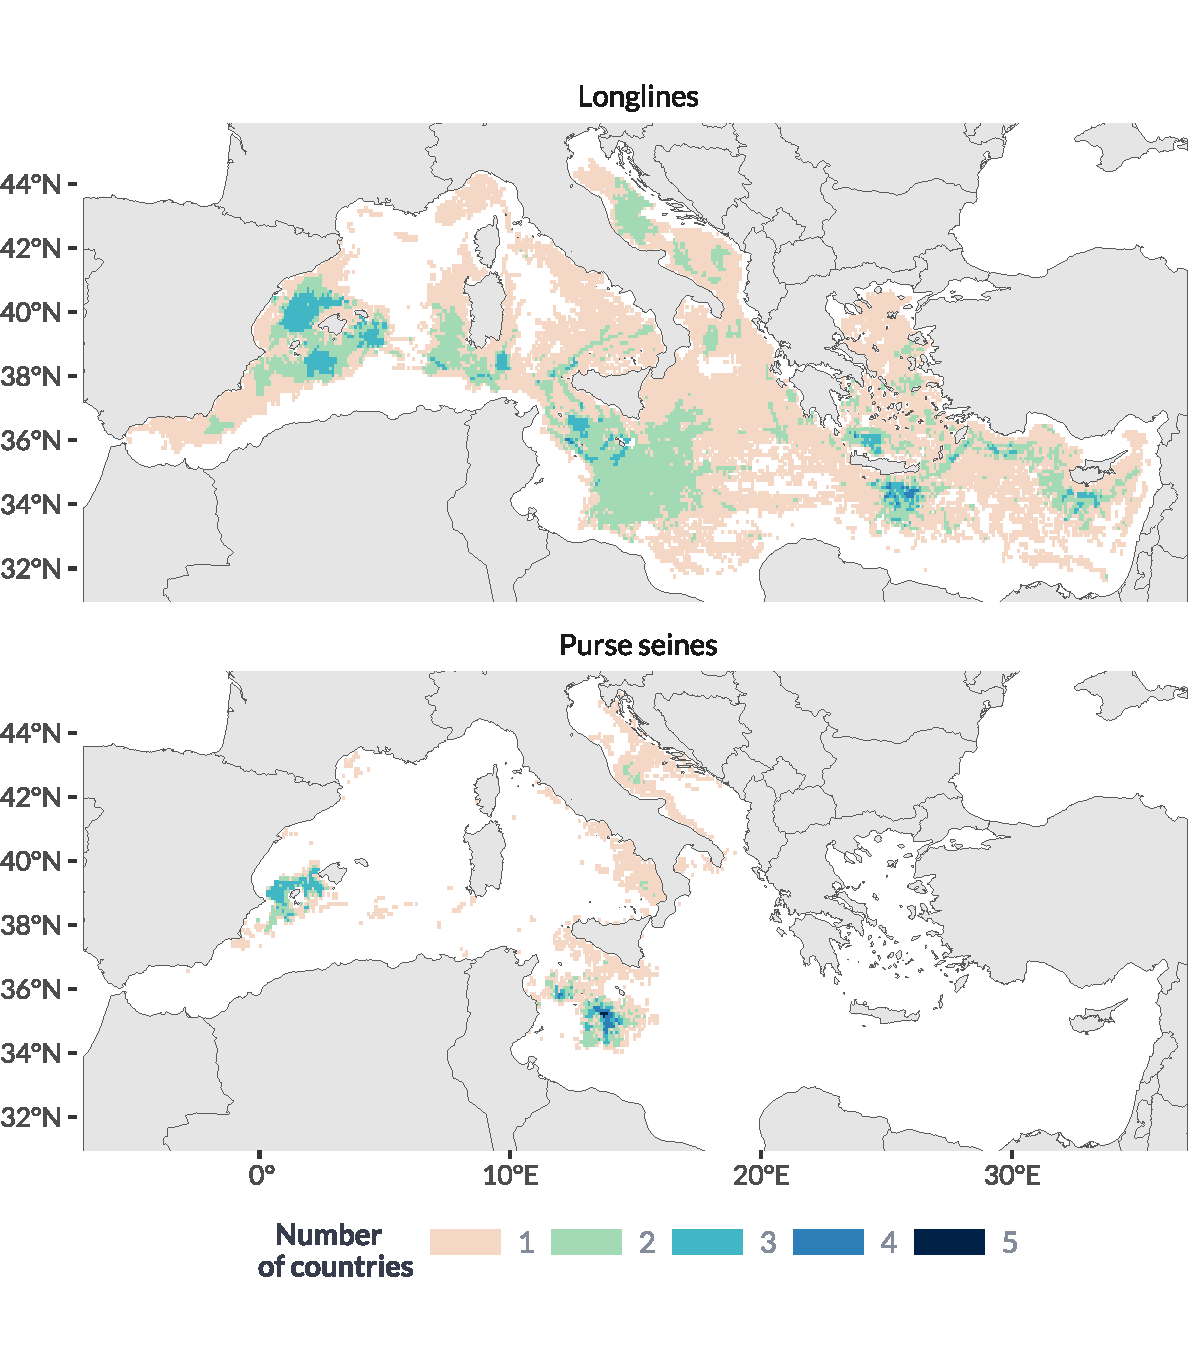
\includegraphics[width=1\linewidth, trim=0 1.2cm 0 1.2cm,clip]{Figures/plots/no_countries.pdf}
	\caption{Number of countries fishing per cell for longliners and purse seiners between 2015-2024.}
	\label{fig:no_countries}
\end{figure}

A comparison of fishing hours from the GFW data with catch data from ICCAT shows that AIS
under-represents fishing activity by non-EU countries relative to EU countries
\figref{fig:ais_iccat}. Even though, many non-EU countries account for a substantial share of the
total reported catches. Notably, AIS also does not capture any French longline vessels.

\begin{figure}[ht]
	\centering
	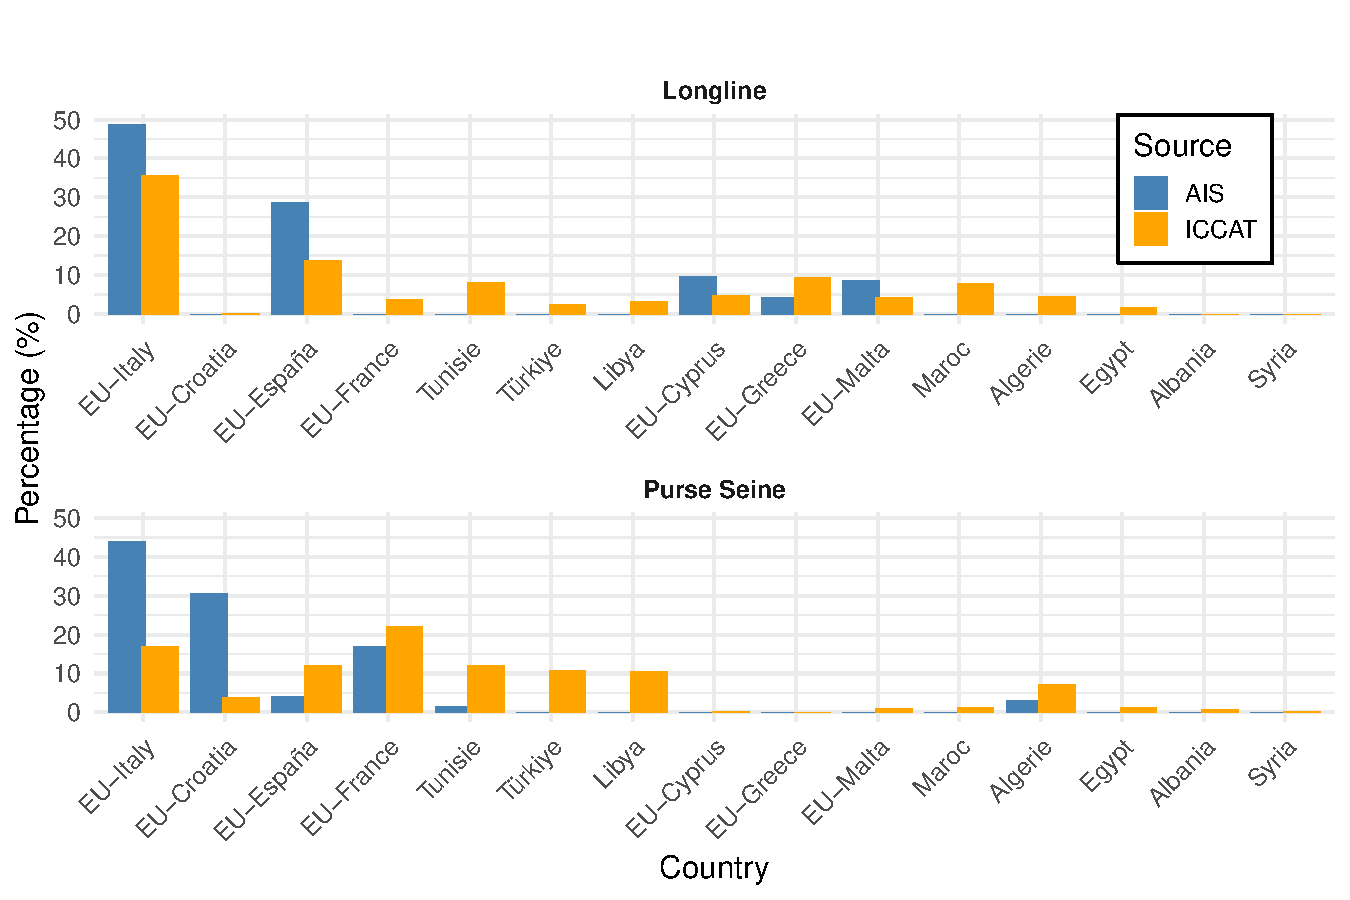
\includegraphics[width=1\linewidth, trim=0 0 0 1cm,clip]{Figures/plots/ais_vs_iccat.pdf}
	\caption{Comparison of relative percentages between GFW AIS data and ICCAT catch data. AIS percentages are relative to the
		total fishing hours between all countries. ICCAT percentages are relative to the total weight of catches between all countries.}
	\label{fig:ais_iccat}
\end{figure}

\FloatBarrier
\section{Depth and distance to port}

The relationship between the cumulative proportion of fishing hours and the distance to port
reveals that most fishing activity of both gear types is concentrated less than 100 km from the
closest port \figref{sub0:fig:depth_dist}. The trend for the depth is different between gear types,
where most purse seine fishing occurs at shallower depths (> 1000 m; 50\% above 500 m depth) and
longline fishing takes place over much greater depth ranges (Fig.~\ref{sub1:fig:depth_dist}; 50\%
above 1600 m depth).

\begin{figure}[ht]
	\customsubplot{2}
	{1\linewidth}                           % width
	{0 0 0 0}                       % trim
	{Figures/plots/depth_dist_both.pdf} % file
	{12,67}                                  % (A) position
	{58,67}                                  % (B) position
	{fig:depth_dist}
	{%
		Cumulative proportion of fishing hours with \subref{sub0:fig:depth_dist}) Distance to port and \subref{sub1:fig:depth_dist}) Depth.}
\end{figure}
